\scanpage{35}
\mspage{\handwritten{3}}
% archive sheet number: 34

\deleted{fermé de $H$),}

\deleted{\uline{\unsure{i)|v)} être un monomorphisme central (6.6),}}

\deleted{\uline{vi) être un monomorphisme invariant (6.6).}}

\inserted{\handwritten{10.4.}} \uline{Soient $j\handwritten{\in}I$, $G_j$ et $H_j$ deux $S_j$-groupes de présentation finie, et $u_j:G_j\handwritten{\longrightarrow}H_j$ un morphisme de $S_j$-groupes. Pour que $u=u_j\handwritten{\times}_{S_j}S$ \deleted{ait la propriété $\handwritten{\mathbb{P}}$} }\inserted{\handwritten{\figure{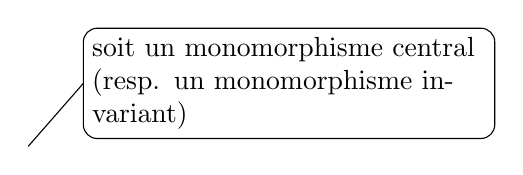
\begin{tikzpicture}
\node[align=left,text width=5cm,inner sep=3pt] (n) at (0,0) {soit un monomorphisme central (resp. un monomorphisme invariant)};
\draw[rounded corners=5pt] (n.south west) rectangle (n.north east);
\draw (n.west) -- ++(-.7,-.8);
\end{tikzpicture}}}}\uline{, il faut et il suffit qu'il existe $i\handwritten{\in}I$, $i\handwritten{\geqslant}j$ tel que $u_i=u_j\handwritten{\times}_{S_j}S_i$ ait la \inserted{\handwritten{même}}propriété $\deleted{\handwritten{\unsure{\mathbb{P}}}}$.}

\deleted{Les assertions (i) à (iv) résultent de (EGA 8.10.5). Les assertions (v) et (vi) sont}\inserted{\handwritten{C'est}} une conséquence immédiate de \deleted{(EGA 8.8.2 et 8.8.3)}\inserted{\handwritten{(10.0) et (10.1),}} compte tenu de la caractérisation donnée en (6.7) des monomorphismes de groupes centraux et invariants.

\inserted{\handwritten{\uline{Corollaire}}} \uuline{10.5.} \uline{Soit $j\handwritten{\in}I$, et soit $G_j$ un $S_j$-groupe de présentation finie. Pour que $G=G_j\handwritten{\times}_{S_j}S$ soit abélien, il faut et il suffit qu'il existe $i\handwritten{\in}I$, $i\handwritten{\geqslant}j$, tel que $G_i=G_j\handwritten{\times}_{S_j}\deleted{\unsure{H}_{\unsure{j|i}}}\inserted{S_i}$ soit abélien.}

En effet, il revient au même de dire qu'un $S$-groupe est abélien, ou que, considéré comme sous-préschéma en groupes de lui-même, il est central.

\uline{Proposition 10.6.}- \uline{Dans la s\unsure{i|à}tuation rappelée au début de (10.0), soient $j\handwritten{\in}I$, $G_j$ un $S_j$-groupe de présentation finie, $G'_j$ un sous-préschéma en groupes de $G_j$ plat et de présentation finie sur $S_j$. Pour que $G_j\handwritten{\times}_{S_j}S/G'_j\handwritten{\times}_{S_j}S$ soit représentable (pour la topologie fpqc), il faut et il suffit qu'il existe $i\handwritten{\in}I$, $i\handwritten{\geqslant}j$, tel que $G_j\handwritten{\times}_{S_j}S_i/G'_j\handwritten{\times}_{S_j}S_i$ soit représentable.}

C'est une conséquence \deleted{p}du lemme plus général suivant :

\margin{\handwritten{$\mathbb{T}$}}
\uline{Lemme 10.7.}- \uline{Soit $\handwritten{\mathbb{T}}$ la topologie fppf ou fpqc; soient $j\handwritten{\in}I$, $X_j$ un $S_j$-préschéma de}
